
\documentclass{article}
\usepackage[headheight=20pt, margin=1.0in, top=1.2in]{geometry}
\usepackage{amsmath, amssymb, amsthm, thmtools, tcolorbox, array, graphicx, makeidx, cancel, multirow, fancyhdr, xypic, color, nicefrac, rotating, multicol, caption, subcaption, xcolor, tikz, tikz-3dplot, tikz-cd, pgfplots, import, enumitem, calc, booktabs, wrapfig, siunitx, hyperref,float}
\hypersetup{colorlinks=true,linkcolor=blue}
\usepackage[all]{xy}
\usepackage{esint}
\setlength{\parindent}{0in}
\sisetup{per-mode = symbol}
\usetikzlibrary{calc,arrows,svg.path,decorations.markings,patterns,matrix,3d,fit}
\usepgfplotslibrary{groupplots}
\pgfplotsset{compat=newest}
\newtcolorbox{mydefbox}[2][]{colback=red!5!white,colframe=red!75!black,fonttitle=\bfseries,title=#2,#1}
\newtcolorbox{mythmbox}[2][]{colback=gray!5!white,colframe=gray!75!black,fonttitle=\bfseries,title=#2,#1}
\newtcolorbox{myexamplebox}[2][]{colback=green!5!white,colframe=green!75!black,fonttitle=\bfseries,title=#2,#1}
\newtcolorbox{mypropbox}[2][]{colback=blue!5!white,colframe=blue!75!black,fonttitle=\bfseries,title=#2,#1}
\declaretheoremstyle[headfont=\color{blue}\normalfont\bfseries,]{colored}
\theoremstyle{definition}
\newtheorem{theorem}{Theorem}
\newtheorem{corollary}[theorem]{Corollary}
\newtheorem{lemma}[theorem]{Lemma}
\newtheorem{proposition}[theorem]{Proposition}
\newtheorem{problem}[theorem]{Problem}
\newtheorem{definition}[theorem]{Definition}
\newtheorem{exercise}[theorem]{Exercise}
\newtheorem{example}[theorem]{Example}
\newtheorem{solution}[theorem]{Solution}
\newtheorem*{thm}{Theorem}
\newtheorem*{lem}{Lemma}
\newtheorem*{prob}{Problem}
\newtheorem*{exer}{Exercise}
\newtheorem*{prop}{Proposition}
\def\R{\mathbb{R}}
\def\F{\mathbb{F}}
\def\Q{\mathbb{Q}}
\def\C{\mathbb{C}}
\def\N{\mathbb{N}}
\def\Z{\mathbb{Z}}
\def\Ra{\Rightarrow}
\def\e{\epsilon}
\newcommand{\typo}[1]{{\color{red}{#1}}}
\newcommand\thedate{\today}
\newcommand{\mb}{\textbf}
\newcommand{\norm}[2]{\|{#1}\|_{#2}}
\newcommand{\normm}[1]{\|#1\|}
\newcommand{\mat}[1]{\begin{bmatrix} #1 \end{bmatrix}}
\newcommand{\eqtext}[1]{\hspace{3mm} \text{#1} \hspace{3mm}}
\newcommand{\set}[1]{\{#1\}}
\newcommand{\inte}{\textrm{int}}
\newcommand{\ra}{\rightarrow}
\newcommand{\minv}{^{-1}}
\newcommand{\tx}[1]{\text{ {#1} }}
\newcommand{\abs}[1]{|#1|}
\newcommand{\mc}[1]{\mathcal{#1}}
\newcommand{\uniflim}{\mathop{\mathrm{unif\lim}}}
\newcommand{\notimplies}{\mathrel{{\ooalign{\hidewidth$\not\phantom{=}$\hidewidth\cr$\implies$}}}}
\pagestyle{fancy}
\fancyhf{}
\fancyhead[L]{Title of the Document}
\fancyhead[C]{}
\fancyhead[R]{\thepage}
\fancyfoot[L]{}
\fancyfoot[C]{}
\fancyfoot[R]{}
\renewcommand{\headrulewidth}{0.4pt}
\renewcommand{\footrulewidth}{0.4pt}
\numberwithin{equation}{section}
% Increase spacing between paragraphs
\setlength{\parskip}{1em}
% Increase spacing before and after sections
\usepackage{titlesec}
\titlespacing*{\section}{0pt}{3ex plus 1ex minus .2ex}{2ex plus .2ex}
\titlespacing*{\subsection}{0pt}{2ex plus 1ex minus .2ex}{1ex plus .2ex}
\titlespacing*{\subsubsection}{0pt}{1ex plus 1ex minus .2ex}{1ex plus .2ex}
\title{\textbf{Title of the Document}}
\author{Author Name}
\date{\today}
\begin{document}
\maketitle
\tableofcontents
\newpage
\section{Exercises}
\begin{enumerate}
    \item Let $(X,d)$ be a metric space and $S \subset X$. Show that $\partial S \subset \overline{S} \cap \overline{S^c}$.
    \item Show that for an arbitrary choice of $a, b, r \in \mathbb{R}$, the closed disk $D = \{(x,y) \mid (x-a)^2 + (y-b)^2 \leq r^2\}$ is a bounded set in $\mathbb{R}^2$.
    \item Let $(X,d)$ be a metric space and for $x,y \in X$. Show that if $d(x,y) < \epsilon$ for every $\epsilon > 0$, then $x = y$.
\end{enumerate}

\subsection*{(i)}

Assume \(\partial S \subseteq \overline{S} \cap \overline{S^c}\).

Then by $x \in \partial S \implies \forall \epsilon > 0: B_\epsilon(x) \cap S^c \neq \emptyset$.

However, by $x \in \partial S$, this value of $\epsilon$ implies

$ B_\epsilon(x) \cap S \neq \emptyset  \Rightarrow B_\epsilon(x) \nsubseteq S $

which is a contradiction, implying our assumption that $x \in \partial S \cap S'$ must be false and

$ \partial S \cap S' = \emptyset $

\subsection*{(ii)}

A set $S$ is bounded if and only if $\exists M \in \mathbb{R}^+ \evry \forall x, y \in S$

$ d(x, y) \leq M $

Let $a, b, r \in \mathbb{R}$.

$ S = \{(x , y) \mid (x - a)^2 + (y - b)^2 \leq r^2\} $

$
\begin{aligned}
    &\implies x^2 - 2ax + a^2 + y^2 - 2yb + b^2 \leq r^2 \\
    &\implies x^2 - 2ax + y^2 - 2yb + r^2 - a^2 - b^2 \\
    &\implies x^2 + y^2 \leq r^2 - a^2 - b^2 + 2ax + 2yb
\end{aligned}
$

We need to show $x^2$ is bounded:

$
\begin{aligned}
    &(x - a)^2 \leq r^2 \\
    &\implies |x - a| \leq |r| \\
    &\implies |x - a| \leq |r| \implies |x| \leq |r| + |a| \\
    &\implies |x| = |x + a - a| \leq |x - a| + |a| \\
    &\implies |x| \leq |r| + |a|
\end{aligned}
$

\subsection*{(iii)}

A set $S$ is bounded if it is contained within some ball, i.e., $\exists M \in \mathbb{R}^+ \ \forall x, y \in S \ \ d(x, y) \leq M$

\begin{center}
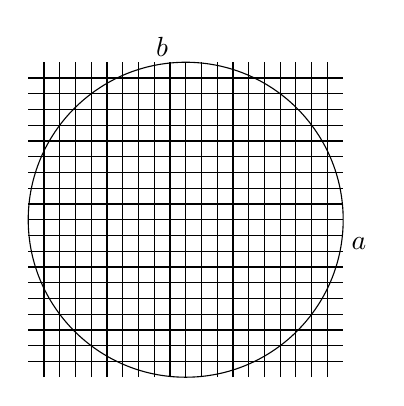
\begin{tikzpicture}
\draw (0,0) circle (2cm);
\draw (0,2) -- (0,-2);
\draw (-2,0) -- (2,0);
\foreach \x in {-1.8,-1.6,...,1.8}
\draw (\x,-2) -- (\x,2);
\foreach \y in {-1.8,-1.6,...,1.8}
\draw (-2,\y) -- (2,\y);
\node at (-0.3,2.2) {\( b \)};
\node at (2.2,-0.3) {\( a \)};
\end{tikzpicture}
\end{center}

$
\Rightarrow \quad |y| \leq r + |a| \quad 
\Rightarrow \quad x^2 \leq (r + |a|)^2
$

\text{Same for } y, \quad y^2 \leq (r + |b|)^2

$
\forall z = (x, y) \in D_{r,a,b}, \quad \|z\| = \sqrt{x^2 + y^2} \leq \sqrt{(r + |a|)^2 + (r + |b|)^2}
$

Thus, if \(\mathcal{M} = \sqrt{(r + |a|)^2 + (r + |b|)^2}\), the bound holds.

\# IS normed boundless = distance boundless.

Let \(x = (x_1, x_2), y = (y_1, y_2) \in D_{r, a, b}\)

$
z_2 \in \{x,y\} \quad (x_2 - a)^2 + (x_2 - b)^2 = r^2 
$

$
\Rightarrow d(z_1, (a,b)) = \sqrt{(x_2 - a)^2 + (x_2 - b)^2} \leq r
$

$
\Rightarrow d(x, y) \leq d(x, (a,b)) + d(y, (a,b)) 
$

$
= \sqrt{(x_1 - a)^2 + (x_1 - b)^2} + \sqrt{(y_1 - a)^2 + (y_1 - b)^2} 
$

$
\leq r + r = 2r.
$

\begin{itemize}
    \item[(iii)] Suppose that \( x \neq y \). Then \( d(x,y) \neq 0 \). Thus if we choose \( \epsilon = d(x,y) \Rightarrow \epsilon > 0 \) but \( d(x,y) \notin \epsilon \). (contradiction).  

    (contradiction) Suppose \( x \neq y \) and so \( d(x,y) \neq 0 \).
    Choose \( \epsilon > 0 \) so that \( \epsilon = d(x,y) \). Then we must have
    $
    d(x,y) < \epsilon = d \left( \frac{d(x,y)}{2} \right) = \frac{d(x,y)}{2}
    $
    which is a contradiction, as this implies
    $
    d(x,y) \leq \frac{d(x,y)}{2}
    \Rightarrow d(x,y) = s < \epsilon = \frac{s}{2}
    \Rightarrow s = s < \frac{s}{2}
    \Rightarrow 2s < s.
    $
    Thus \( x = y \).

    \item[(iv)] Let \( (V, \| \cdot \|) \) be a normed vsp. Then let \( r > 0 \) and \( x \in V \). Then
    $
    B_r(x) = \{ u \in V \mid d(x,u) < r \}
    $
    $
    B_{r + \| x \|}(0) = \{ v \in V \mid d(0,v) < r + \| x \| \}
    $

    \begin{center}
    % \includegraphics{diagram.png} % Note: Add the diagram here.
    \end{center}

    Let \( y \in B_r(x) \).

    $
    d(0,y) \leq d(0,x) + d(x,y)
    $
    $
    d(0,y) \leq \| x \| + r
    $

    $
    \Rightarrow B_r(x) \subseteq B_{r+\| x \|}(0)
    $

    \item[(v)] Suppose \( S \) is bounded. Then \( \exists M \in \mathbb{R} : \forall x \in S \| x \| \leq M \).

    (Equiv to \( \exists M > 0 : \forall x \in V \))
    $
    x \in B_M(0)
    $
\end{itemize}\end{document}